% Stanford Gemini Poster — pdfLaTeX compatible
% Compiler: pdfLaTeX (default on Overleaf)

\documentclass[final]{beamer}

\usepackage[T1]{fontenc}
\usepackage{lmodern}
\usepackage[size=custom,width=101.6,height=76.2,scale=1.0]{beamerposter}
\usetheme{gemini}
\usecolortheme{stanford}
\usepackage{graphicx}
\usepackage{booktabs}
\usepackage{tikz}
\usepackage{amsmath}
\usepackage{amssymb}
\usepackage{array}
\usepackage{enumitem}

\graphicspath{{figures/}{overleaf_submission/figures/}}

% ====================
% Lengths — 3 columns
% ====================
\newlength{\sepwidth}
\newlength{\colwidth}
\setlength{\sepwidth}{0.020\paperwidth}
\setlength{\colwidth}{0.313\paperwidth}

\newcommand{\separatorcolumn}{\begin{column}{\sepwidth}\end{column}}

\setlength{\abovecaptionskip}{0.2ex}
\setlength{\belowcaptionskip}{0ex}
\setlist{nosep, leftmargin=1.5em, topsep=0pt, itemsep=1pt, parsep=0pt}

% ====================
% Title / Authors
% ====================
\title{Decoupling What from Where: Action-Type-Conditioned Grounding for GUI Agents}
\author{Aadi Chauhan \and Arthur Ilyasov}
\institute[Stanford]{Stanford University \quad CS 231N, Spring 2026}

\footercontent{
  CS 231N: Deep Learning for Computer Vision \hfill
  Stanford University, Spring 2026 \hfill
  \{aadic, ailyasov\}@stanford.edu
}

\begin{document}

\addtobeamertemplate{headline}{}
{
  \begin{tikzpicture}[remember picture,overlay]
    \node [anchor=north east, inner sep=1.4cm]
      at ([xshift=0.0cm,yshift=1.4cm]current page.north east)
      {
\includegraphics[height=4.8cm]{Block_S_2_color.png}};
  \end{tikzpicture}
}

\begin{frame}[t]
\begin{columns}[t]
\separatorcolumn

% ============================================================
% COLUMN 1
% ============================================================
\begin{column}{\colwidth}

  \begin{block}{Motivation: The Compounding-Error Problem}
    GUI agents must predict an \textbf{action type} (\emph{click, scroll, type, \ldots}) and a \textbf{pixel-level target} from a screenshot and instruction. State-of-the-art models (UI-TARS, OS-Atlas, SeeClick) emit both in one autoregressive decode, entangling the two sub-problems.

    \textbf{Failure mode:} Committing to the wrong action type causes coherent-but-wrong grounding: the model clicks precisely within the wrong semantic region. On long-horizon tasks these errors compound --- each mistyped action corrupts screen state for every subsequent step.

    \textbf{Our question:} Does explicitly factoring action-type prediction from spatial grounding reduce this error? We show it does, but the \emph{mechanism} that captures the benefit is not the one we hypothesized.

    \begin{figure}
      \centering
      
\includegraphics[width=\linewidth]{qualitative_grounding.png}
      \caption{Qualitative grounding examples. Conditioned model (right) correctly targets the intended element; flat baseline (left) grounds in the wrong semantic region of the screen.}
    \end{figure}
  \end{block}

  \begin{block}{Two-Stage Pipeline}
    \heading{Stage 1 --- Action-Type Classifier}
    A \textbf{frozen} Qwen2-VL-2B backbone extracts mean-pooled visual + text features; a 3-layer MLP classifies the action type (click / scroll / type). Vision is critical on AITW ($+0.414$ macro-F1 over text-only) but negligible on Mind2Web ($+0.009$), because AITW instructions describe \emph{goals} rather than explicitly naming the action. Stage 1 achieves \textbf{0.843 accuracy, 0.795 macro-F1} with no extra backbone cost at inference.

    \heading{Stage 2 --- Conditioned Grounder}
    A LoRA-fine-tuned Qwen2-VL-2B predicts the coordinate \texttt{(x,y)} on a 0--999 grid, conditioned on the Stage~1 action-type prediction via one of five mechanisms (A through D-token, described in the center column). The oracle$\to$predicted end-to-end gap is only $\approx\!0.02$ hit@0.10 --- classifier error is not the bottleneck.

    \begin{figure}
      \centering
      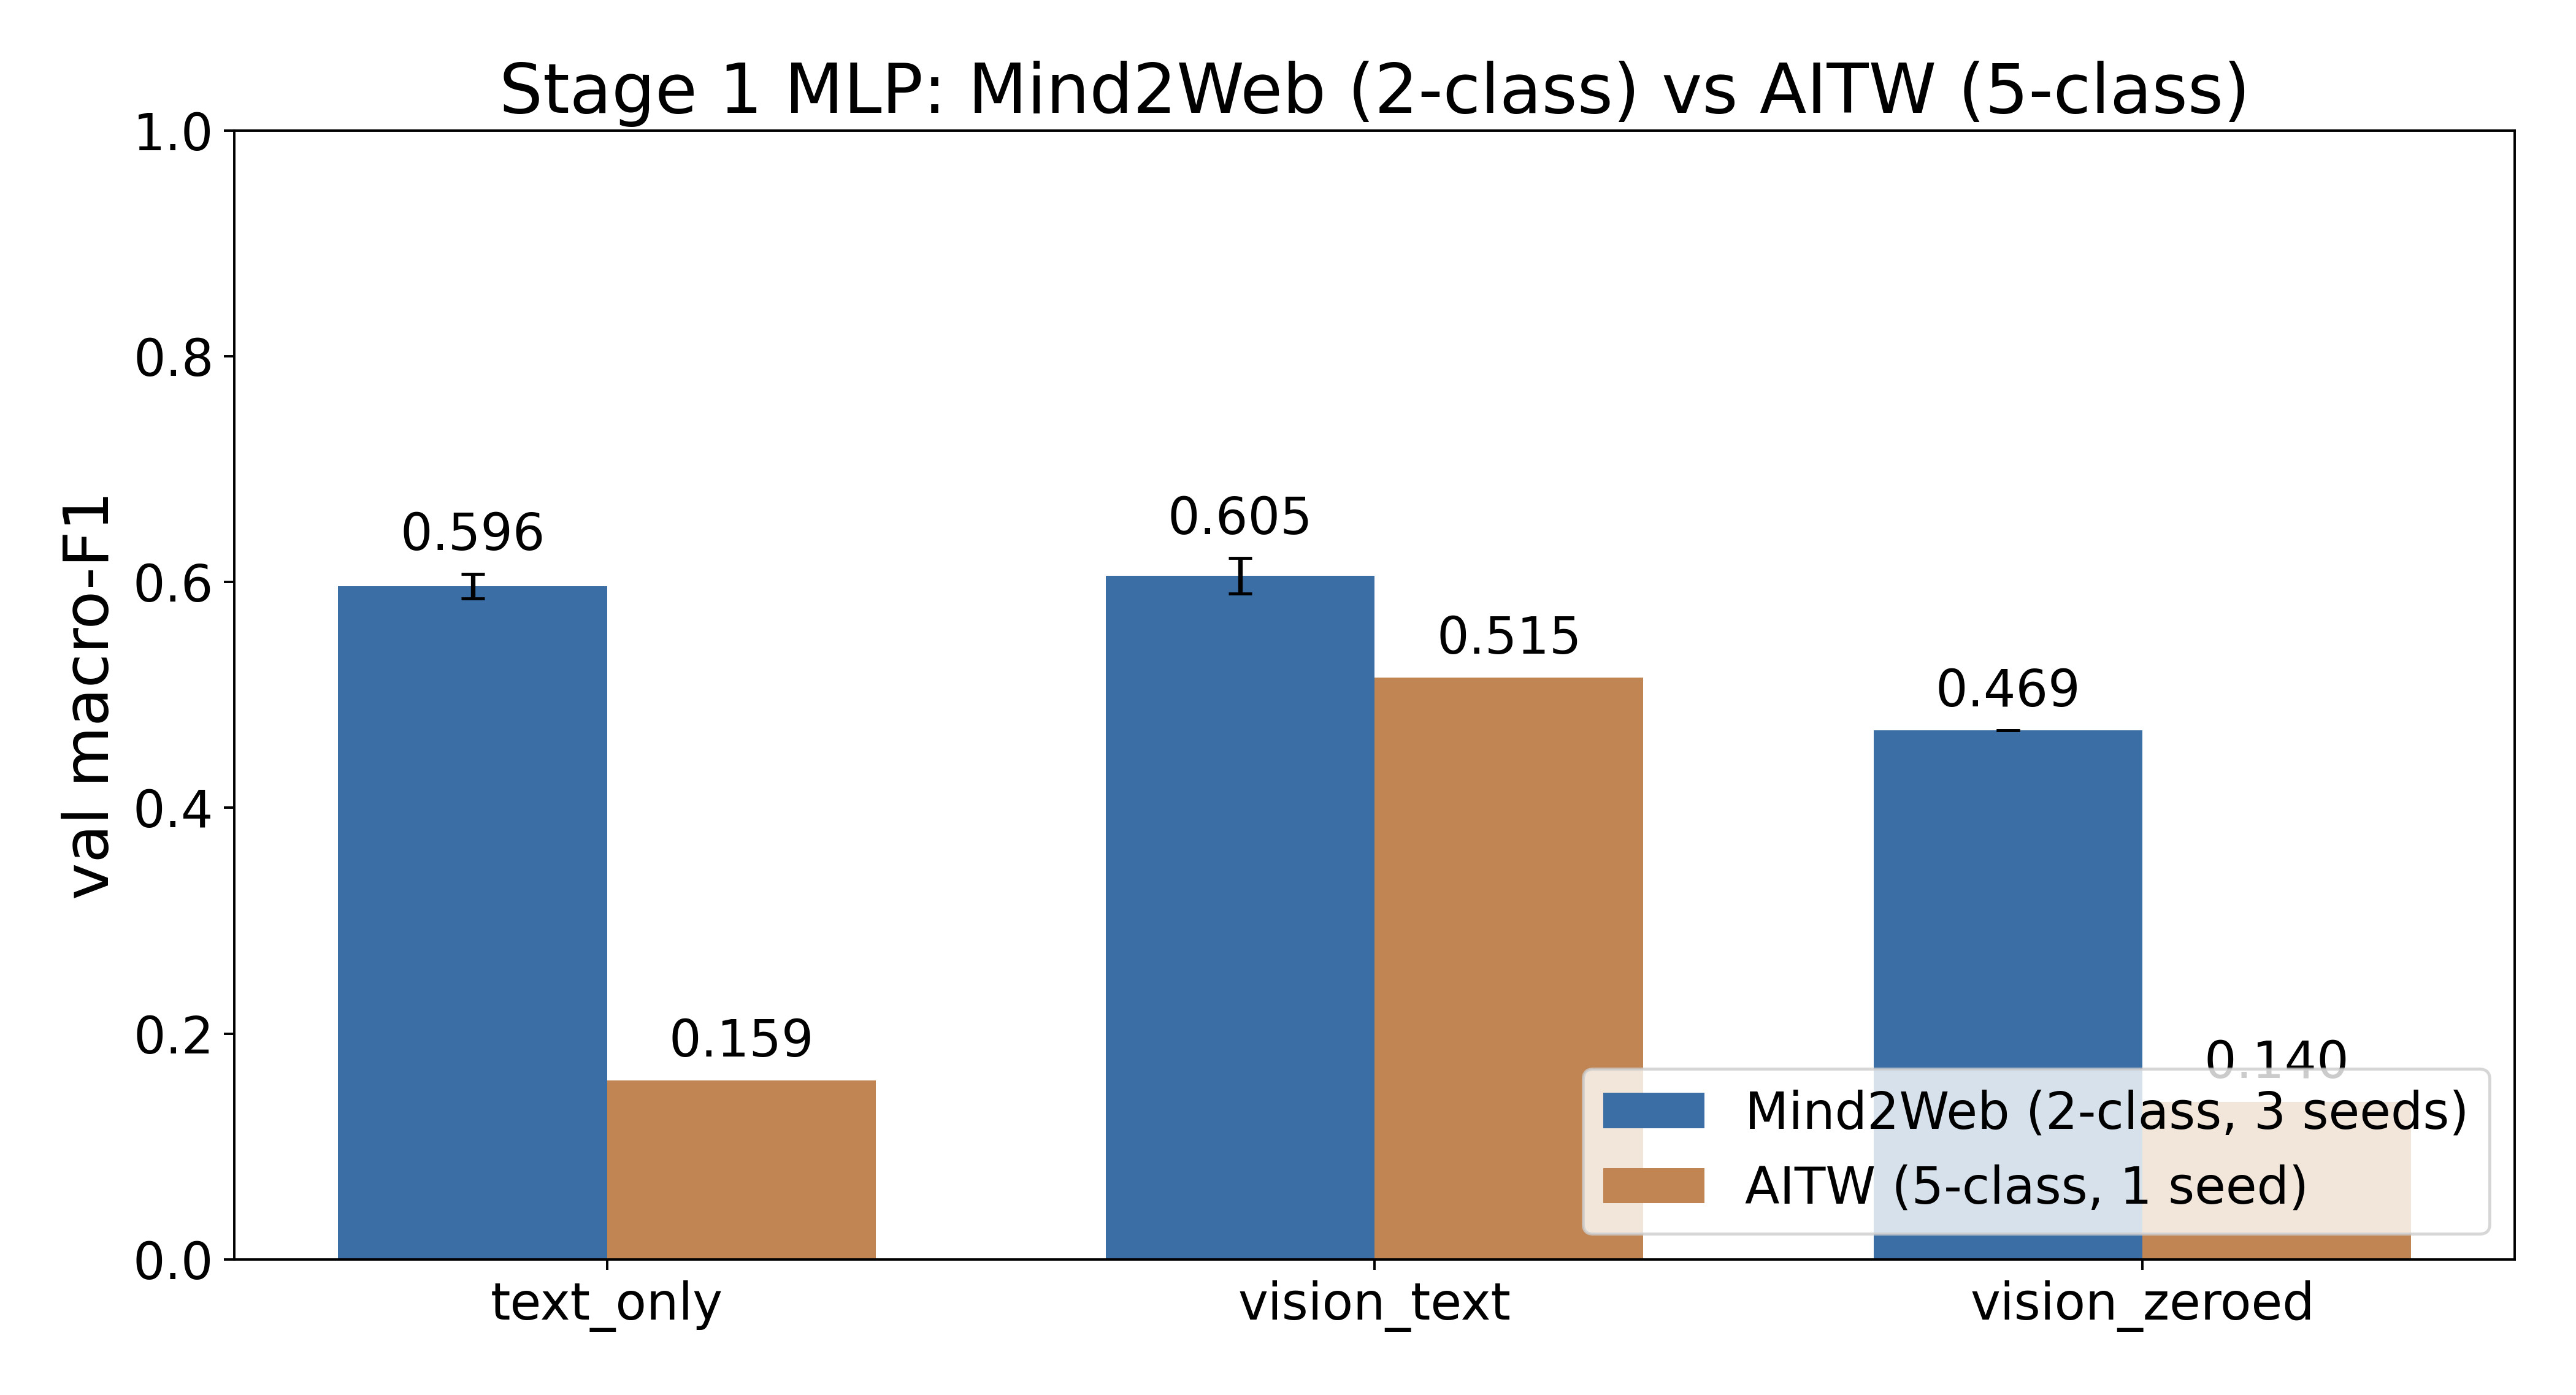
\includegraphics[width=\linewidth]{stage1_mind2web_vs_aitw.png}
      \caption{Stage~1 macro-F1 on Mind2Web vs.\ AITW across modalities. The large vision gain on AITW ($+0.414$) confirms that screenshots carry strong action-type signal when instructions describe task goals.}
    \end{figure}
  \end{block}

\end{column}
\separatorcolumn

% ============================================================
% COLUMN 2
% ============================================================
\begin{column}{\colwidth}

  \begin{block}{Five Stage-2 Conditioning Mechanisms}
    All five variants share identical data, optimizer, backbone (Qwen2-VL-2B + LoRA), and evaluation; only the conditioning mechanism changes.

    \begin{tabular}{@{}lp{0.72\linewidth}@{}}
      \toprule
      \textbf{Var.} & \textbf{Mechanism} \\
      \midrule
      \textbf{A} & Flat baseline --- plain prompt $\to$ coords; no action signal anywhere \\[0.15ex]
      \textbf{B} & Auxiliary action-type classification head (joint loss); action signal at training time only \\[0.15ex]
      \textbf{C} & Hard routing --- emit \texttt{\{word\} (x,y)} format; gold action word forced at decode \\[0.15ex]
      \textbf{D-hook} & Additive action embedding hook, broadcast to all input token positions \\[0.15ex]
      \textbf{D-token} & Dedicated \texttt{<|action\_slot|>} prepended token; learned embedding, M-RoPE-correct \\
      \bottomrule
    \end{tabular}
  \end{block}

  \begin{alertblock}{Main Results --- all\_with\_coords (Spatially Informative)}
    AITW Stage~2 grounding, $n_{\text{train}}=1200$, 3 seeds, Qwen2-VL-2B + LoRA:

    \begin{tabular}{@{}lcccc@{}}
      \toprule
      \textbf{Variant} & \textbf{hit@0.05} & \textbf{hit@0.10} & \textbf{hit@0.25} & \textbf{L2$\downarrow$} \\
      \midrule
      A (flat)        & 0.148 & 0.255$\pm$0.021 & 0.515 & 0.392 \\
      \textbf{B}      & 0.177 & \textbf{0.305$\pm$0.012} & \textbf{0.585} & \textbf{0.362} \\
      C               & 0.148 & 0.279$\pm$0.032 & 0.543 & 0.412 \\
      \textbf{D-hook} & 0.177 & \textbf{0.300$\pm$0.028} & \textbf{0.569} & \textbf{0.365} \\
      D-token         & 0.175 & 0.269$\pm$0.025 & 0.533 & 0.375 \\
      \bottomrule
    \end{tabular}

    Paired bootstrap ($n{=}750$): \textbf{B and D-hook beat A on all metrics} ($p{<}0.002$). \textbf{Ranking: B $\approx$ D-hook $>$ D-token $\gtrsim$ C $>$ A.}
  \end{alertblock}

  \begin{block}{Control --- taps\_and\_swipes (Not Spatially Informative)}
    When action type carries no spatial signal, conditioning is neutral to harmful --- confirming the benefit is mechanism-specific, not a general training artifact.

    \begin{tabular}{@{}lccc@{}}
      \toprule
      \textbf{Variant} & \textbf{hit@0.10} & \textbf{hit@0.25} & \textbf{L2$\downarrow$} \\
      \midrule
      A (flat)   & \textbf{0.390$\pm$0.008} & 0.727 & 0.184 \\
      B          & 0.368$\pm$0.009 & 0.730 & \textbf{0.173} \\
      C          & 0.325$\pm$0.032 & 0.635 & 0.271 \\
      D-hook     & 0.392$\pm$0.035 & 0.723 & 0.179 \\
      \bottomrule
    \end{tabular}
  \end{block}

  \begin{block}{Ablation Summary}
    \begin{figure}
      \centering
      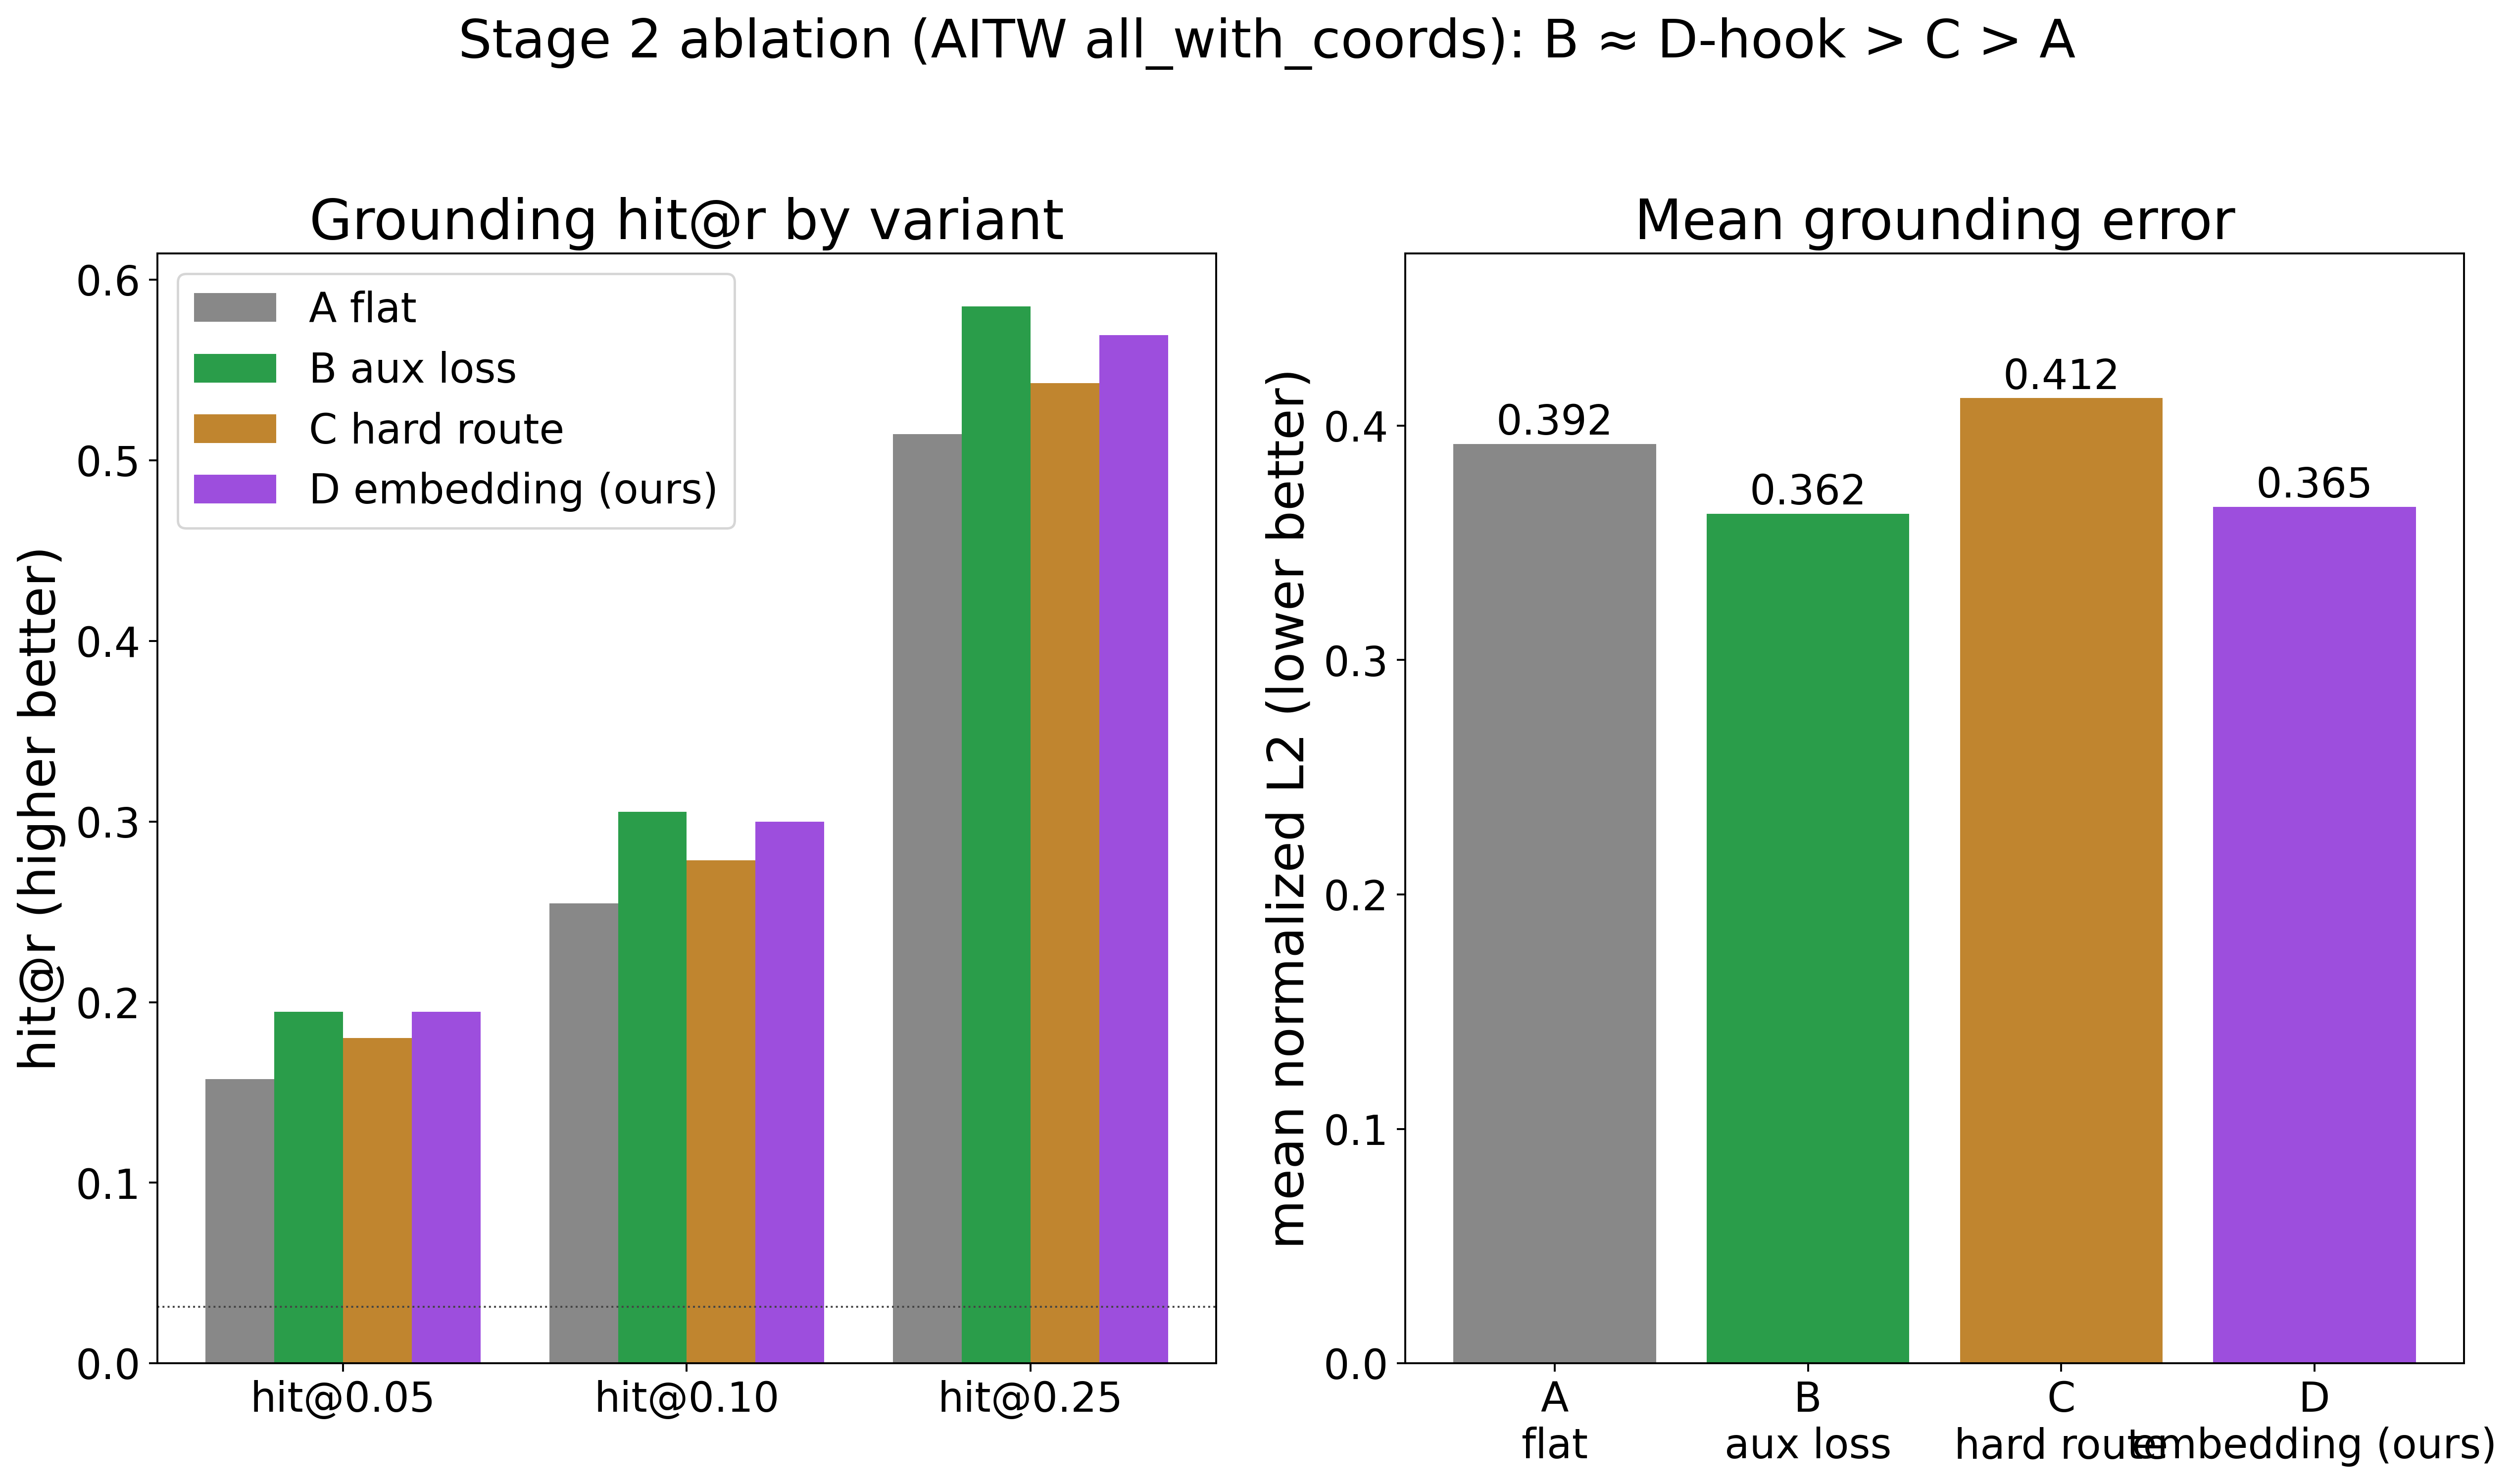
\includegraphics[width=\linewidth]{ablation_ABCD_all_with_coords.png}
      \caption{Hit@0.10 across all five variants on \texttt{all\_with\_coords} (mean$\pm$std, 3 seeds). B and D-hook significantly outperform the flat baseline A; D-token and C trail despite using richer conditioning signals.}
    \end{figure}
  \end{block}

\end{column}
\separatorcolumn

% ============================================================
% COLUMN 3
% ============================================================
\begin{column}{\colwidth}

  \begin{block}{Where Does Conditioning Help?}
    Breaking results by action type reveals the gain is entirely in \textbf{click} (68\% of val). \texttt{type} actions score 0.000 on every variant --- AITW stores a fixed degenerate coordinate for type events, making them ungroundable.

    \begin{figure}
      \centering
      
\includegraphics[width=\linewidth,height=11cm,keepaspectratio]{compounding_error_per_class.png}
      \caption{Hit@0.10 by action type. The conditioning advantage is concentrated in \emph{click}; \texttt{scroll} is split; \texttt{type} is degenerate.}
    \end{figure}

    \begin{tabular}{@{}lcccc@{}}
      \toprule
      \textbf{Action} & \textbf{A} & \textbf{B$-$A} & \textbf{D-hook$-$A} & \textbf{C$-$A} \\
      \midrule
      click (68\%) & 0.253 & \textbf{+0.120} & +0.058 & +0.122 \\
      scroll (18\%) & 0.313 & $-$0.023 & \textbf{+0.039} & $-$0.144 \\
      type (14\%)  & 0.000 & 0.000 & 0.000 & 0.000 \\
      \bottomrule
    \end{tabular}

    The signal is \textbf{click-vs-scroll/type disambiguation}, not field localization. C wins click ($+0.122$) but destroys scroll ($-0.144$), explaining its mediocre overall score.
  \end{block}

  \begin{block}{Low-Data Regime \& Scaling}
    \begin{figure}
      \centering
      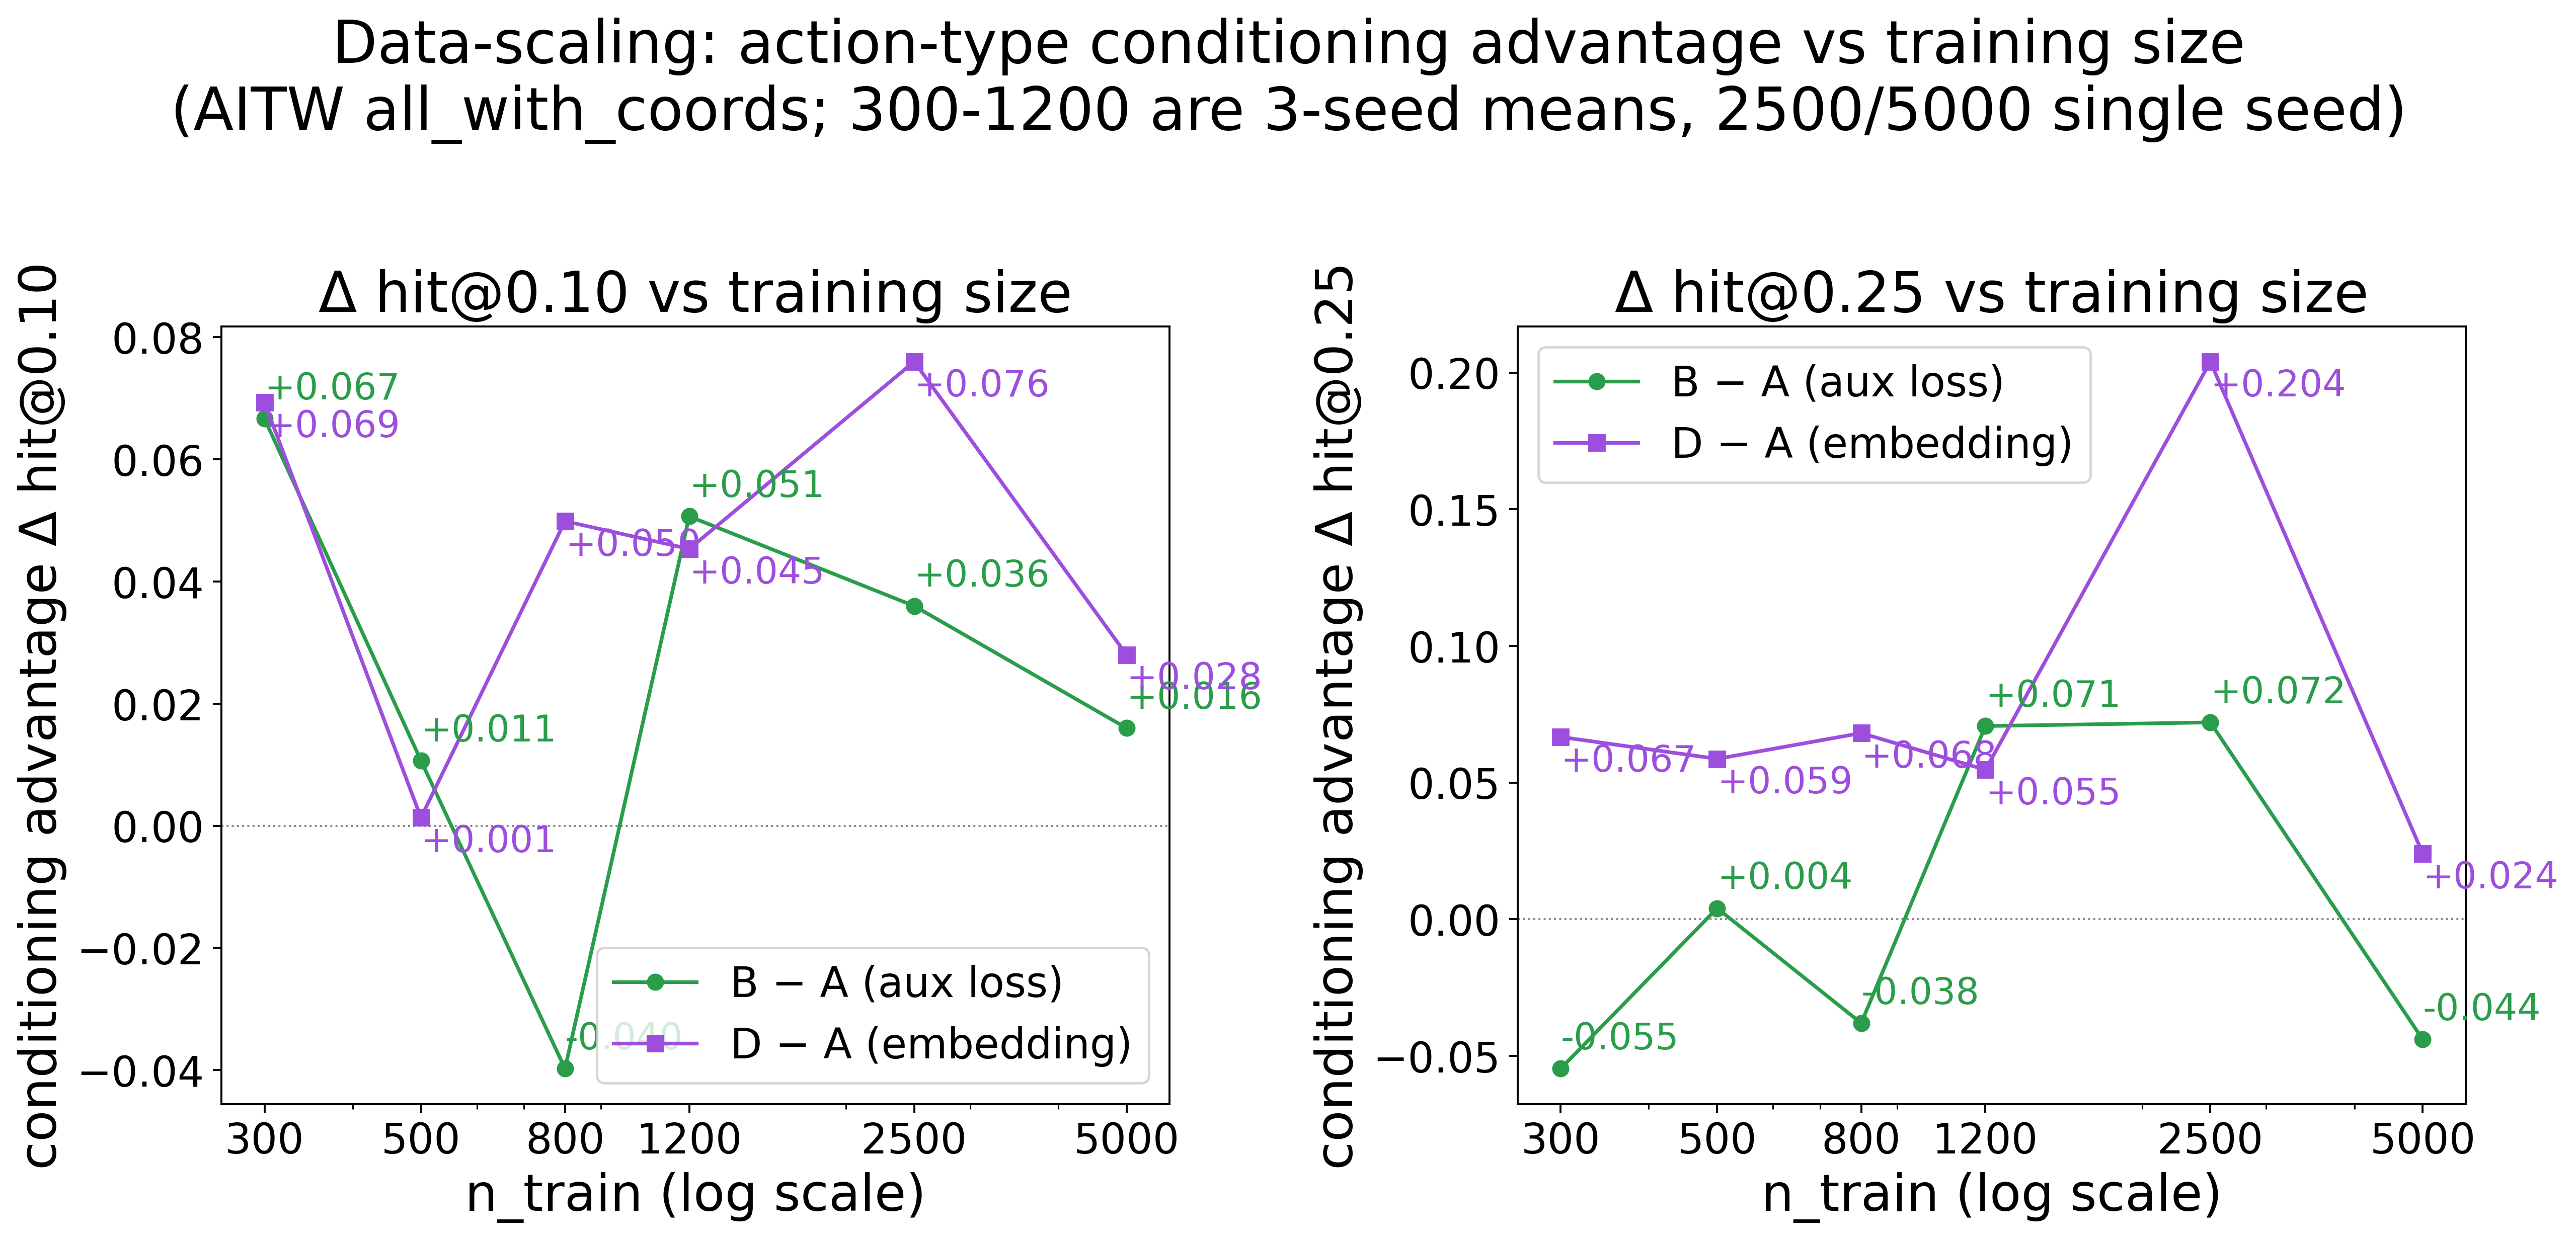
\includegraphics[width=\linewidth,height=10cm,keepaspectratio]{scaling_curve.png}
      \caption{Conditioning advantage vs.\ $n_\text{train}$. Gap largest at $n{=}300$, shrinks at $n{=}5000$ --- action-type supervision is a \textbf{low-data prior} absorbed at scale.}
    \end{figure}

    \begin{tabular}{@{}rcc@{}}
      \toprule
      $n_\text{train}$ & B$-$A (hit@0.10) & D-hook$-$A \\
      \midrule
      300  & +0.067 & +0.069 \\
      1200 & +0.051 & +0.045 \\
      5000 & +0.016 & +0.028 \\
      \bottomrule
    \end{tabular}

    \textbf{D-token causal test:} wrong action id drops hit@0.10 from 0.276$\to$0.084 ($\Delta{=}{+}0.192$, $p{<}0.001$); zeroed embedding also drops to 0.183. The embedding is causally used at inference --- the refutation is ``\emph{used but not best},'' not ``ignored.''
  \end{block}

  \begin{alertblock}{Conclusions}
    \begin{itemize}
      \item \textbf{Broad thesis supported:} B and D-hook beat flat A ($p{<}0.002$) when action type is spatially predictive; effect vanishes on the taps/swipes control and on Mind2Web.
      \item \textbf{Architectural claim refuted:} Auxiliary loss B is the best variant; the hypothesized prepended embedding D-token does not beat B/D-hook on headline metrics despite being causally used.
      \item \textbf{Mechanism:} Click-vs-scroll/type disambiguation, largest at low data.
      \item \textbf{Pitfall:} \texttt{inputs\_embeds} bypass of Qwen2-VL M-RoPE produces $8\sigma$ false negative --- fixed by preserving \texttt{input\_ids}.
    \end{itemize}
  \end{alertblock}

  \begin{block}{References}
    \scriptsize
    \begin{enumerate}[leftmargin=1.8em, label={[\arabic*]}, itemsep=0pt, topsep=0pt, parsep=0pt]
      \item Yao et al. \textit{UI-TARS: Pioneering Automated GUI Interaction.} arXiv:2501.12326, 2025.
      \item Wu et al. \textit{OS-Atlas: A Foundation Action Model for Generalist GUI Agents.} arXiv:2410.23218, 2024.
      \item Cheng et al. \textit{SeeClick: Harnessing GUI Grounding.} arXiv:2401.10935, 2024.
      \item Deng et al. \textit{Mind2Web: Towards a Generalist Agent for the Web.} NeurIPS, 2023.
      \item Rawles et al. \textit{Android in the Wild.} NeurIPS, 2023.
      \item Wang et al. \textit{Qwen2-VL: Enhancing Vision-Language Model Perception.} arXiv:2409.12191, 2024.
    \end{enumerate}
  \end{block}

\end{column}
\separatorcolumn
\end{columns}
\end{frame}
\end{document}
